%************************************************
\chapter{Column Chromatography (Introduction)}
%************************************************
\begin{flushright}
January 21, 2013
\end{flushright}
\section{Aim}
To get a hands on experience with the Column Chromatography technique, using a single compound, viz. p-Nitro Aniline.

\section {Chemicals Required}
	\begin{enumerate}
		\item Silica
		\item Iodine
		\item Ethyl Acetate
		\item Benzene
		\item p-Nitro Aniline (given compound, refer to \autoref{e3_compound})
	\end{enumerate}

	\begin{figure}[bth]
		\begin{center}
			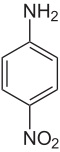
\includegraphics[width=0.1\linewidth]{gfx/e3_compound}
		\end{center}
	\caption[p-Nitroanline]{\label{e3_compound}}
	\end{figure}


\section{Theory}
	TLC is good for detecting what constitutes a mixture. However its yield is very little. To overcome this difficulty, we use a technique known as ``Column Chromatography''. The principle of differential binding of compounds with the solvent is still harnessed. However, instead of relying on the capillary action, we now rely on gravity. The setup consists of a vertical wet (hexane) silica column, contained in a suitable glass container with a flow control apparatus and a nozzle at the bottom. The compound (if solid, then first dissolved in an appropriate solvent) is added on top of the silica column and on top of it the eluent (a suitably polar solution) is added. This moves down through the silica column, differentially moving the constituents of the mixture (which is just a compound in our case). Then if the compound is visible, we can easily use this property and collect the constituents in different test tubes. However, if the compounds are not visible, we may need to run a TLC for each small volume collected.
	\par
	Wikipedia has a very concise and accurate description of the same, which can also be referred to.


\section{Procedure}	
	\begin{enumerate}
		\item Determining the concentration of Elluent to use
		\begin{enumerate}
			\item Prepared the TLC plates as in the previous experiments
			\item Setup the Visibility Chamber, again as before
			\item Various concentrations ($50\%$, $30\%$ and $20\%$) Ethyl Acetate Soln. in Hexane were created
			\item The given compound was diluted in Ethyl Acetate.
			\item TLC was run using the given compound for the various concentrations, till the $R_f$ value was found to be less than $\frac 1 2$, just as described in the previous experiments. \marginpar {\Lisa This step helps determine the kind of solution we use for the elluent as it determines the speed at which the separation process will take place.}
			\item Use the concentration value for which the TLC is roughly less then half, as the Elluent's concentration. This was found to be $20\%$ for our case as is given in the next section.
		\end{enumerate}
		\item Preparing the Wet Column
		\begin{enumerate}
			\item While the TLCs run, a slurry of silica was created in hexane (with about 20-30 spatula of silica) and it was poured in glass column, as described in the theory.
			\item To this, hexane was added, and it was shaken until all air bubbles disappeared. Further the volume of hexane was reduced to about $1$ cm above the silica gel alongside, by allowing hexane to flow through the nozzle.
			\item The compound, along with silica, were mixed with ethyl acetate to form a thick slurry.
			\item This mixture was transferred on top of the silica column.
			\item After it settled reasonably, cotton was added to further level and to ensure that addition of elluent doesn't disturb the mixture (in this case the compound). This ensures that when the separation process proceeds, it doesn't happen out of plane (with respect to the cross section of the container)
		\end{enumerate}
		\item Running the Column
		\begin{enumerate}
			\item Got a set of ordered test tubes in a suitable holder.
			\item The Elluent was poured into the glass column cautiously and sealed from the top.
			\item The liquid was allowed to flow through the nozzle of the glass column, into the test tubes, progressively, as they filled.
			\item For various test tubes, TLC was run again to find its composition. However, since the compound was coloured, this process was initiated only when the test tubes were known to visibly contain the compound (as could be readily seen from the column as time progressed).
		\end{enumerate}


	\end{enumerate}
\section{Observations and Results}		
	To find the concentration of Elluent to use, please refer to \autoref{e3_init}. We obtained the following results
	\begin{enumerate}
		\item With $50\%$ $R_f$ = 0.85
		\item With $30\%$ $R_f$ = 0.62
		\item With $20\%$ $R_f$ = 0.25
	\end{enumerate}

	\begin{figure}[bth]
		\begin{center}
			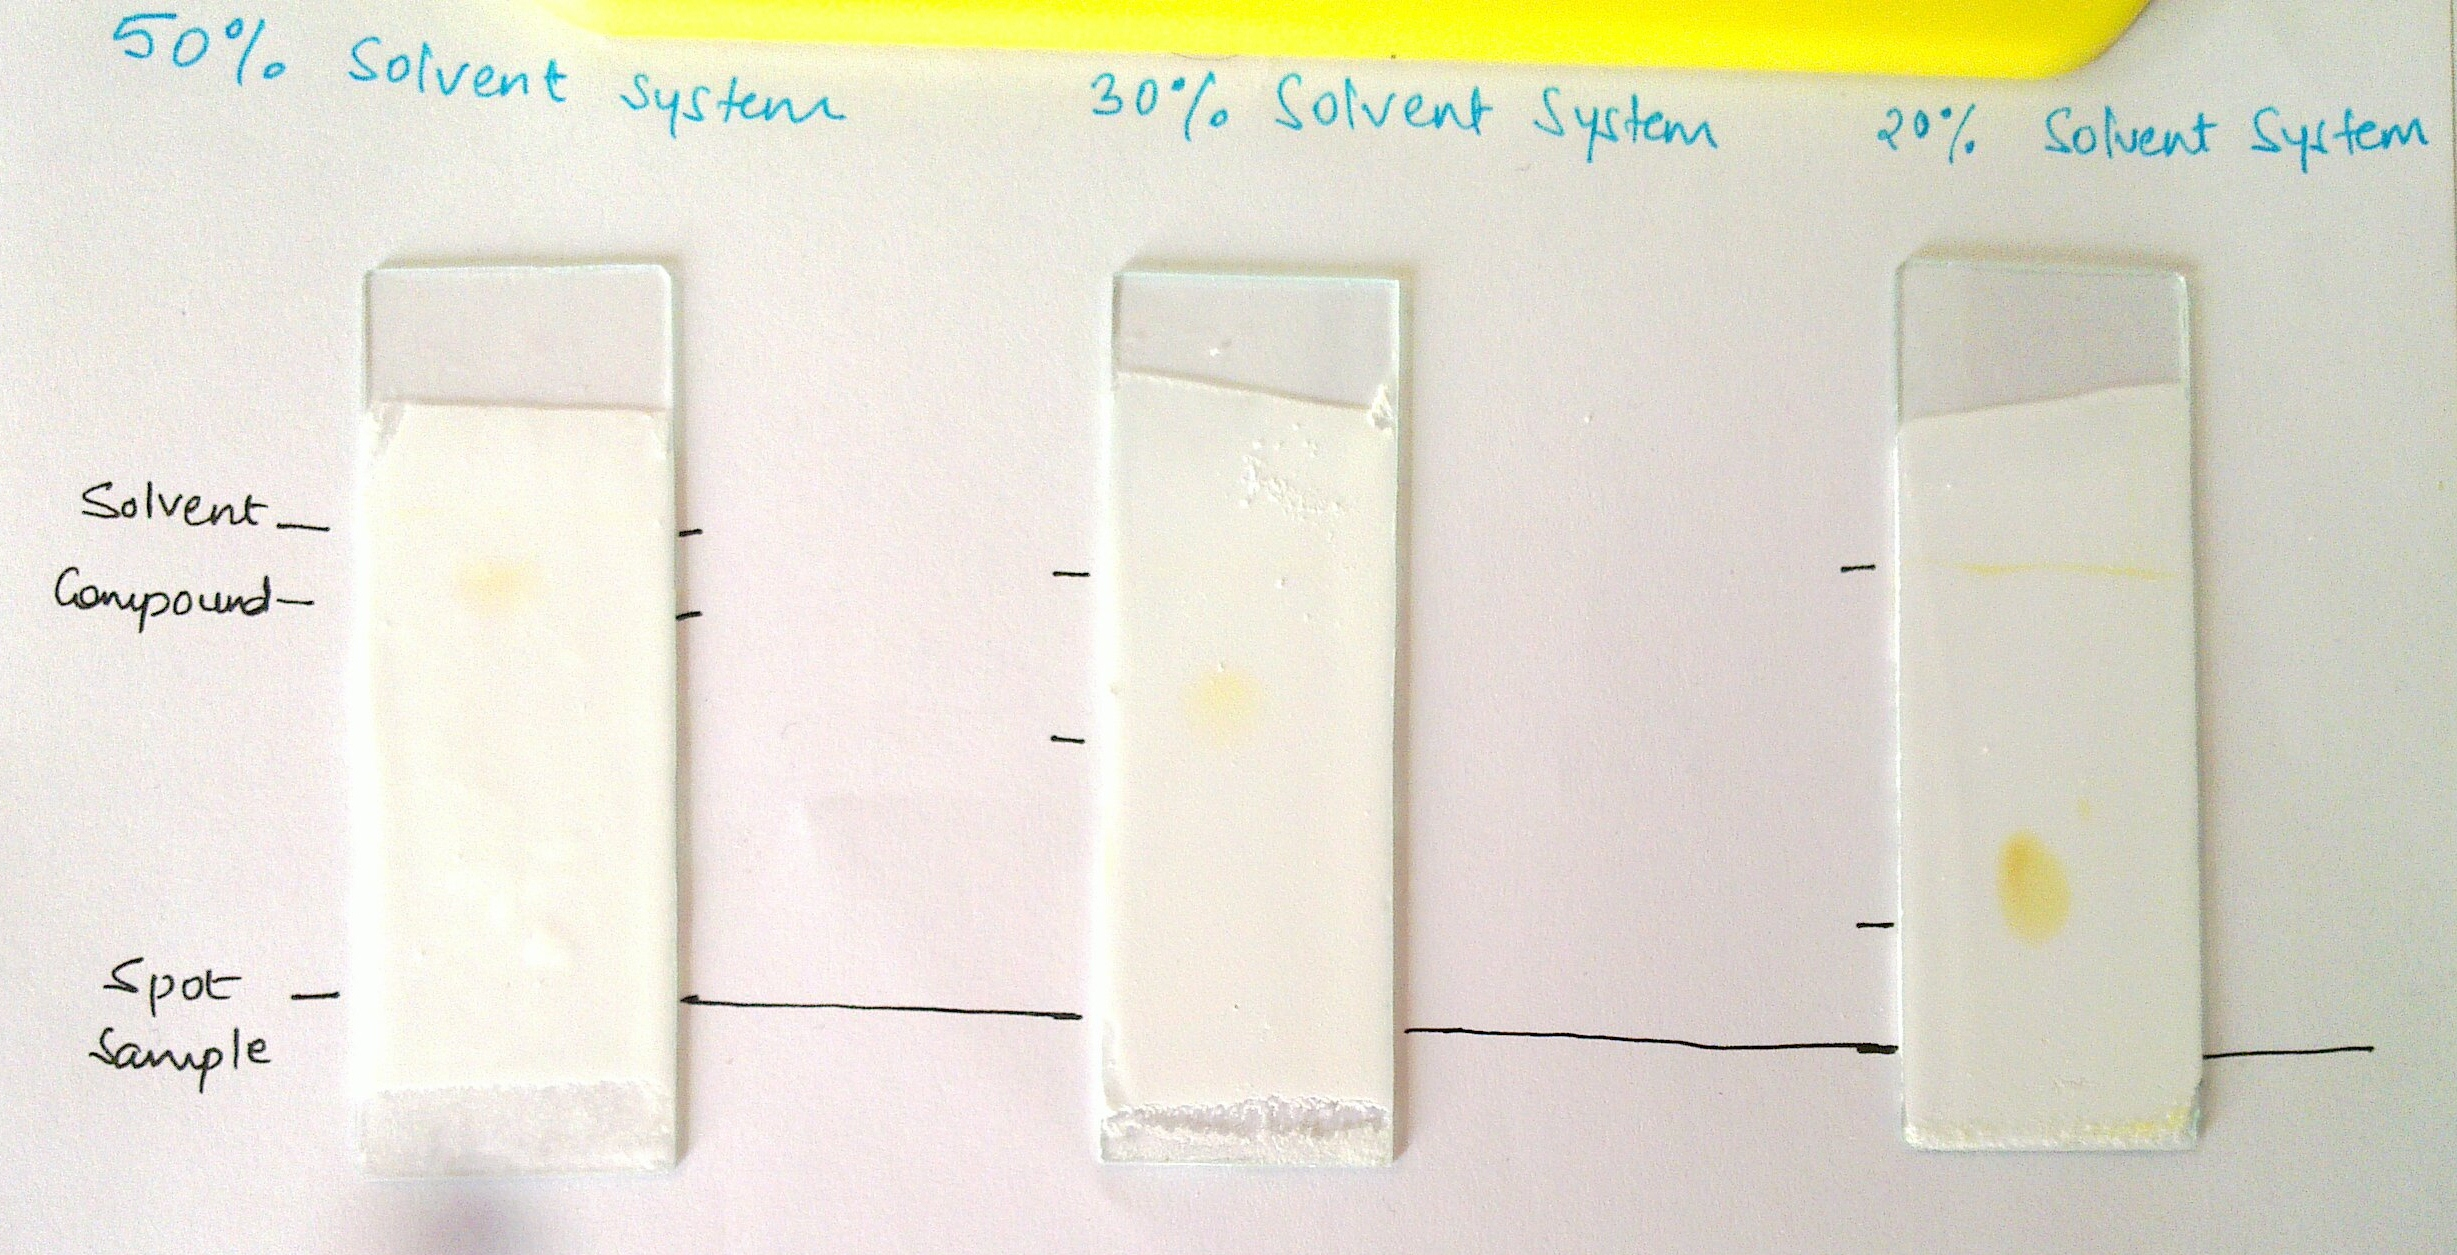
\includegraphics[width=1.2\linewidth]{gfx/e3_init}
		\end{center}
	\caption[TLC plates for the Initial Run]{\label{e3_init}}
	\end{figure}

	To find the constituents of the test tubes, we run TLC with a $20\%$ system, on each of them and the results are as follows. Refer to \autoref{e3_first} and \autoref{e3_second} for details.
	\begin{enumerate}
		\item Plate 1, $R_f$=0.17
		\item Plate 2, $R_f$=0.18
		\item Plate 3, $R_f$=0.21
		\item *Plate 4, $R_f$=0.27
		\item Plate 5, $R_f$=0.18
		\item *Plate 8, $R_f$=0.10
		\item Plate 10, $R_f$=0.17
		\item Plate 11, $R_f$=0.15
	\end{enumerate}
	* appear to be outliers
	Since the mixture consists of only one compound, we expect to get the same $R_f$ values for all coloured test tubes, which seems to hold good for the first place of decimal.
	


	\begin{figure}[bth]
		\begin{center}
			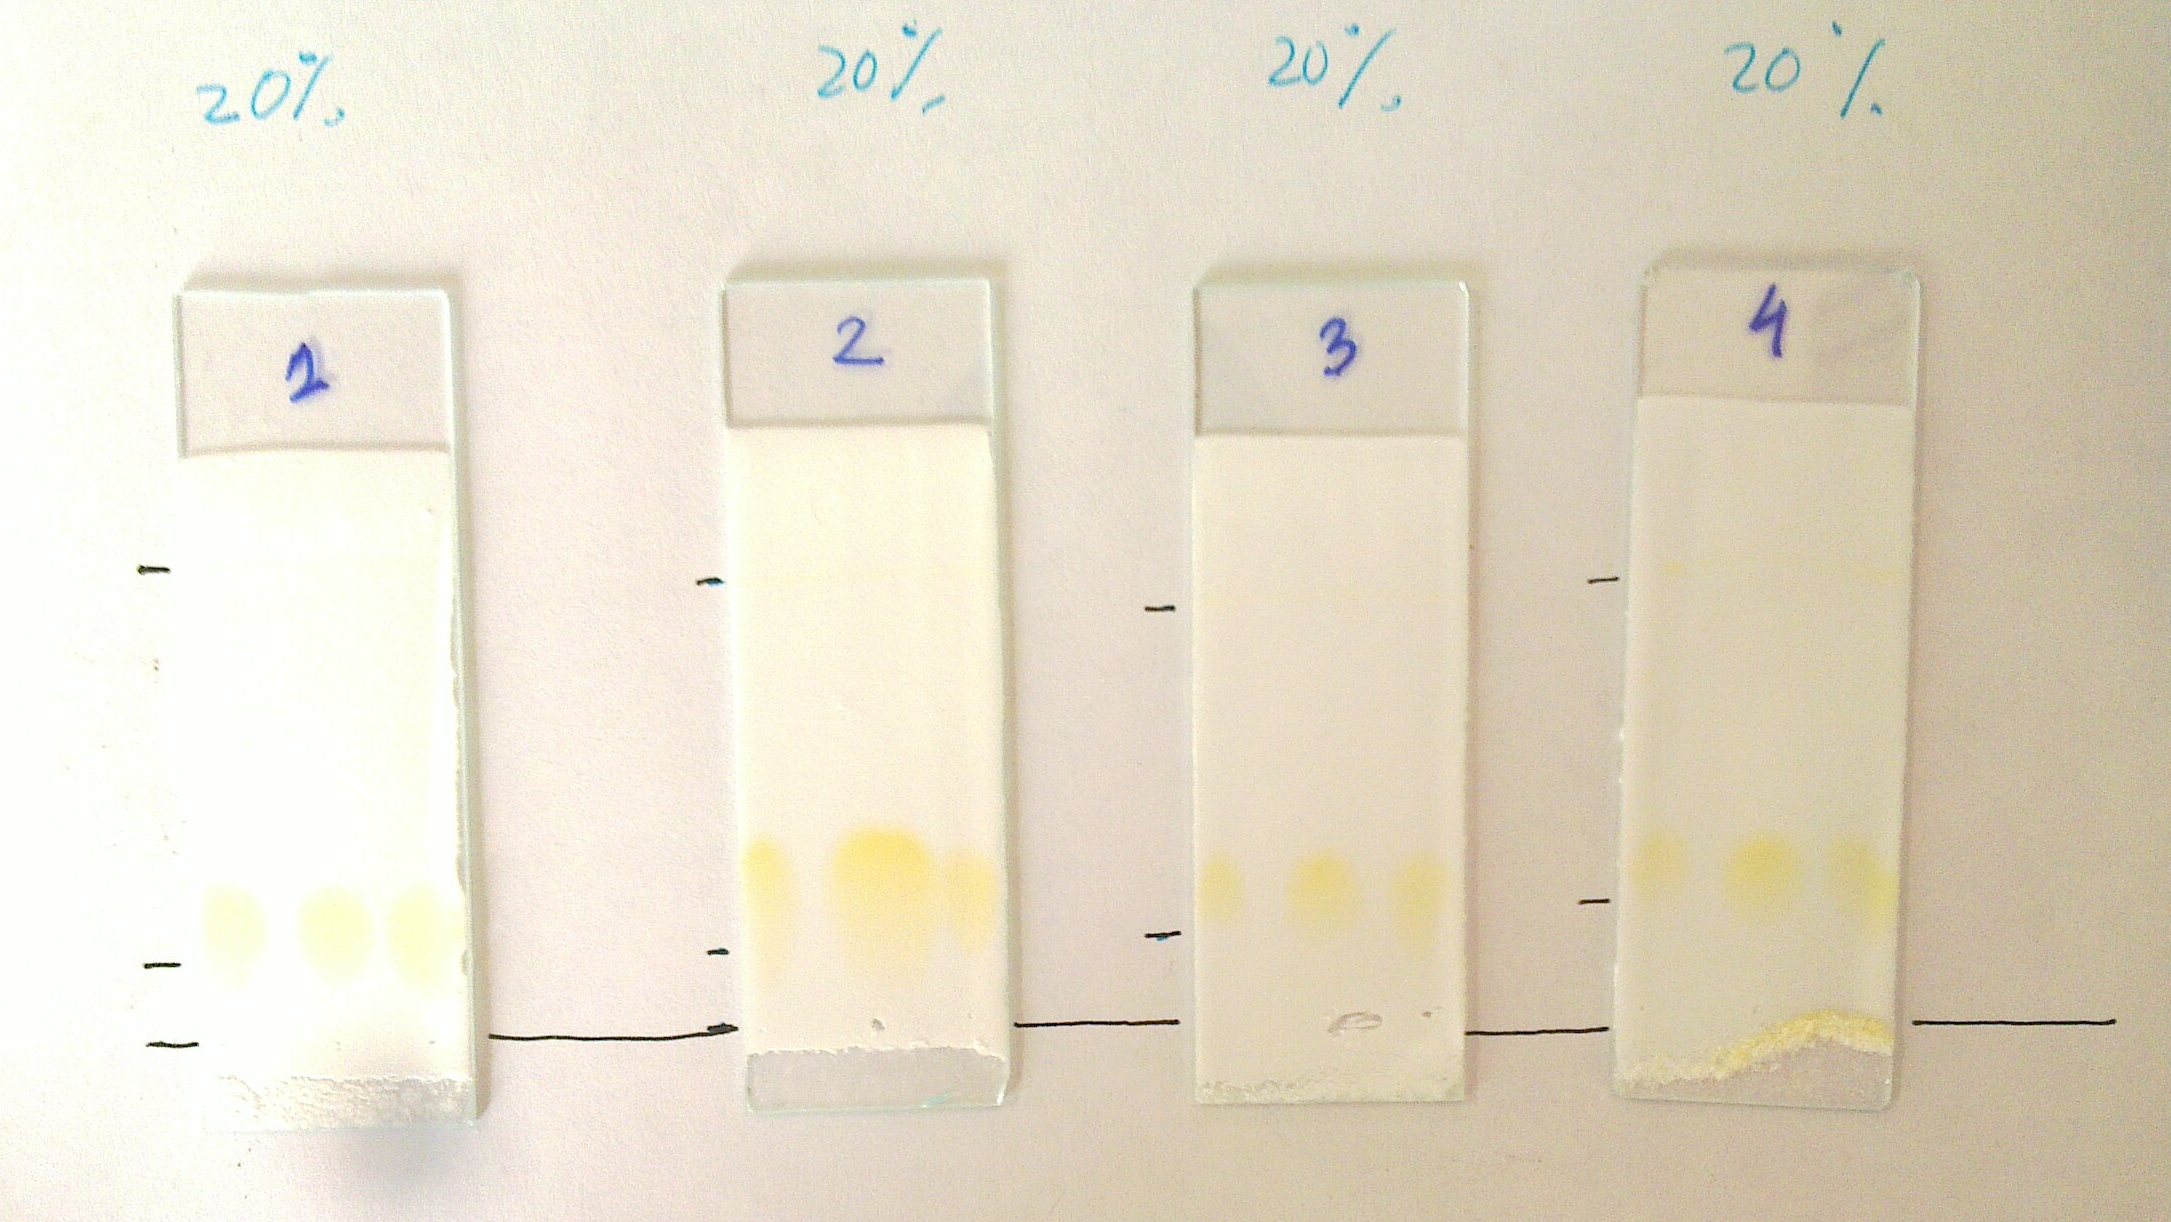
\includegraphics[width=1.2\linewidth]{gfx/e3_first}
		\end{center}
	\caption[TLC plates for various test tubes]{\label{e3_first}}
	\end{figure}

	\begin{figure}[bth]
		\begin{center}
			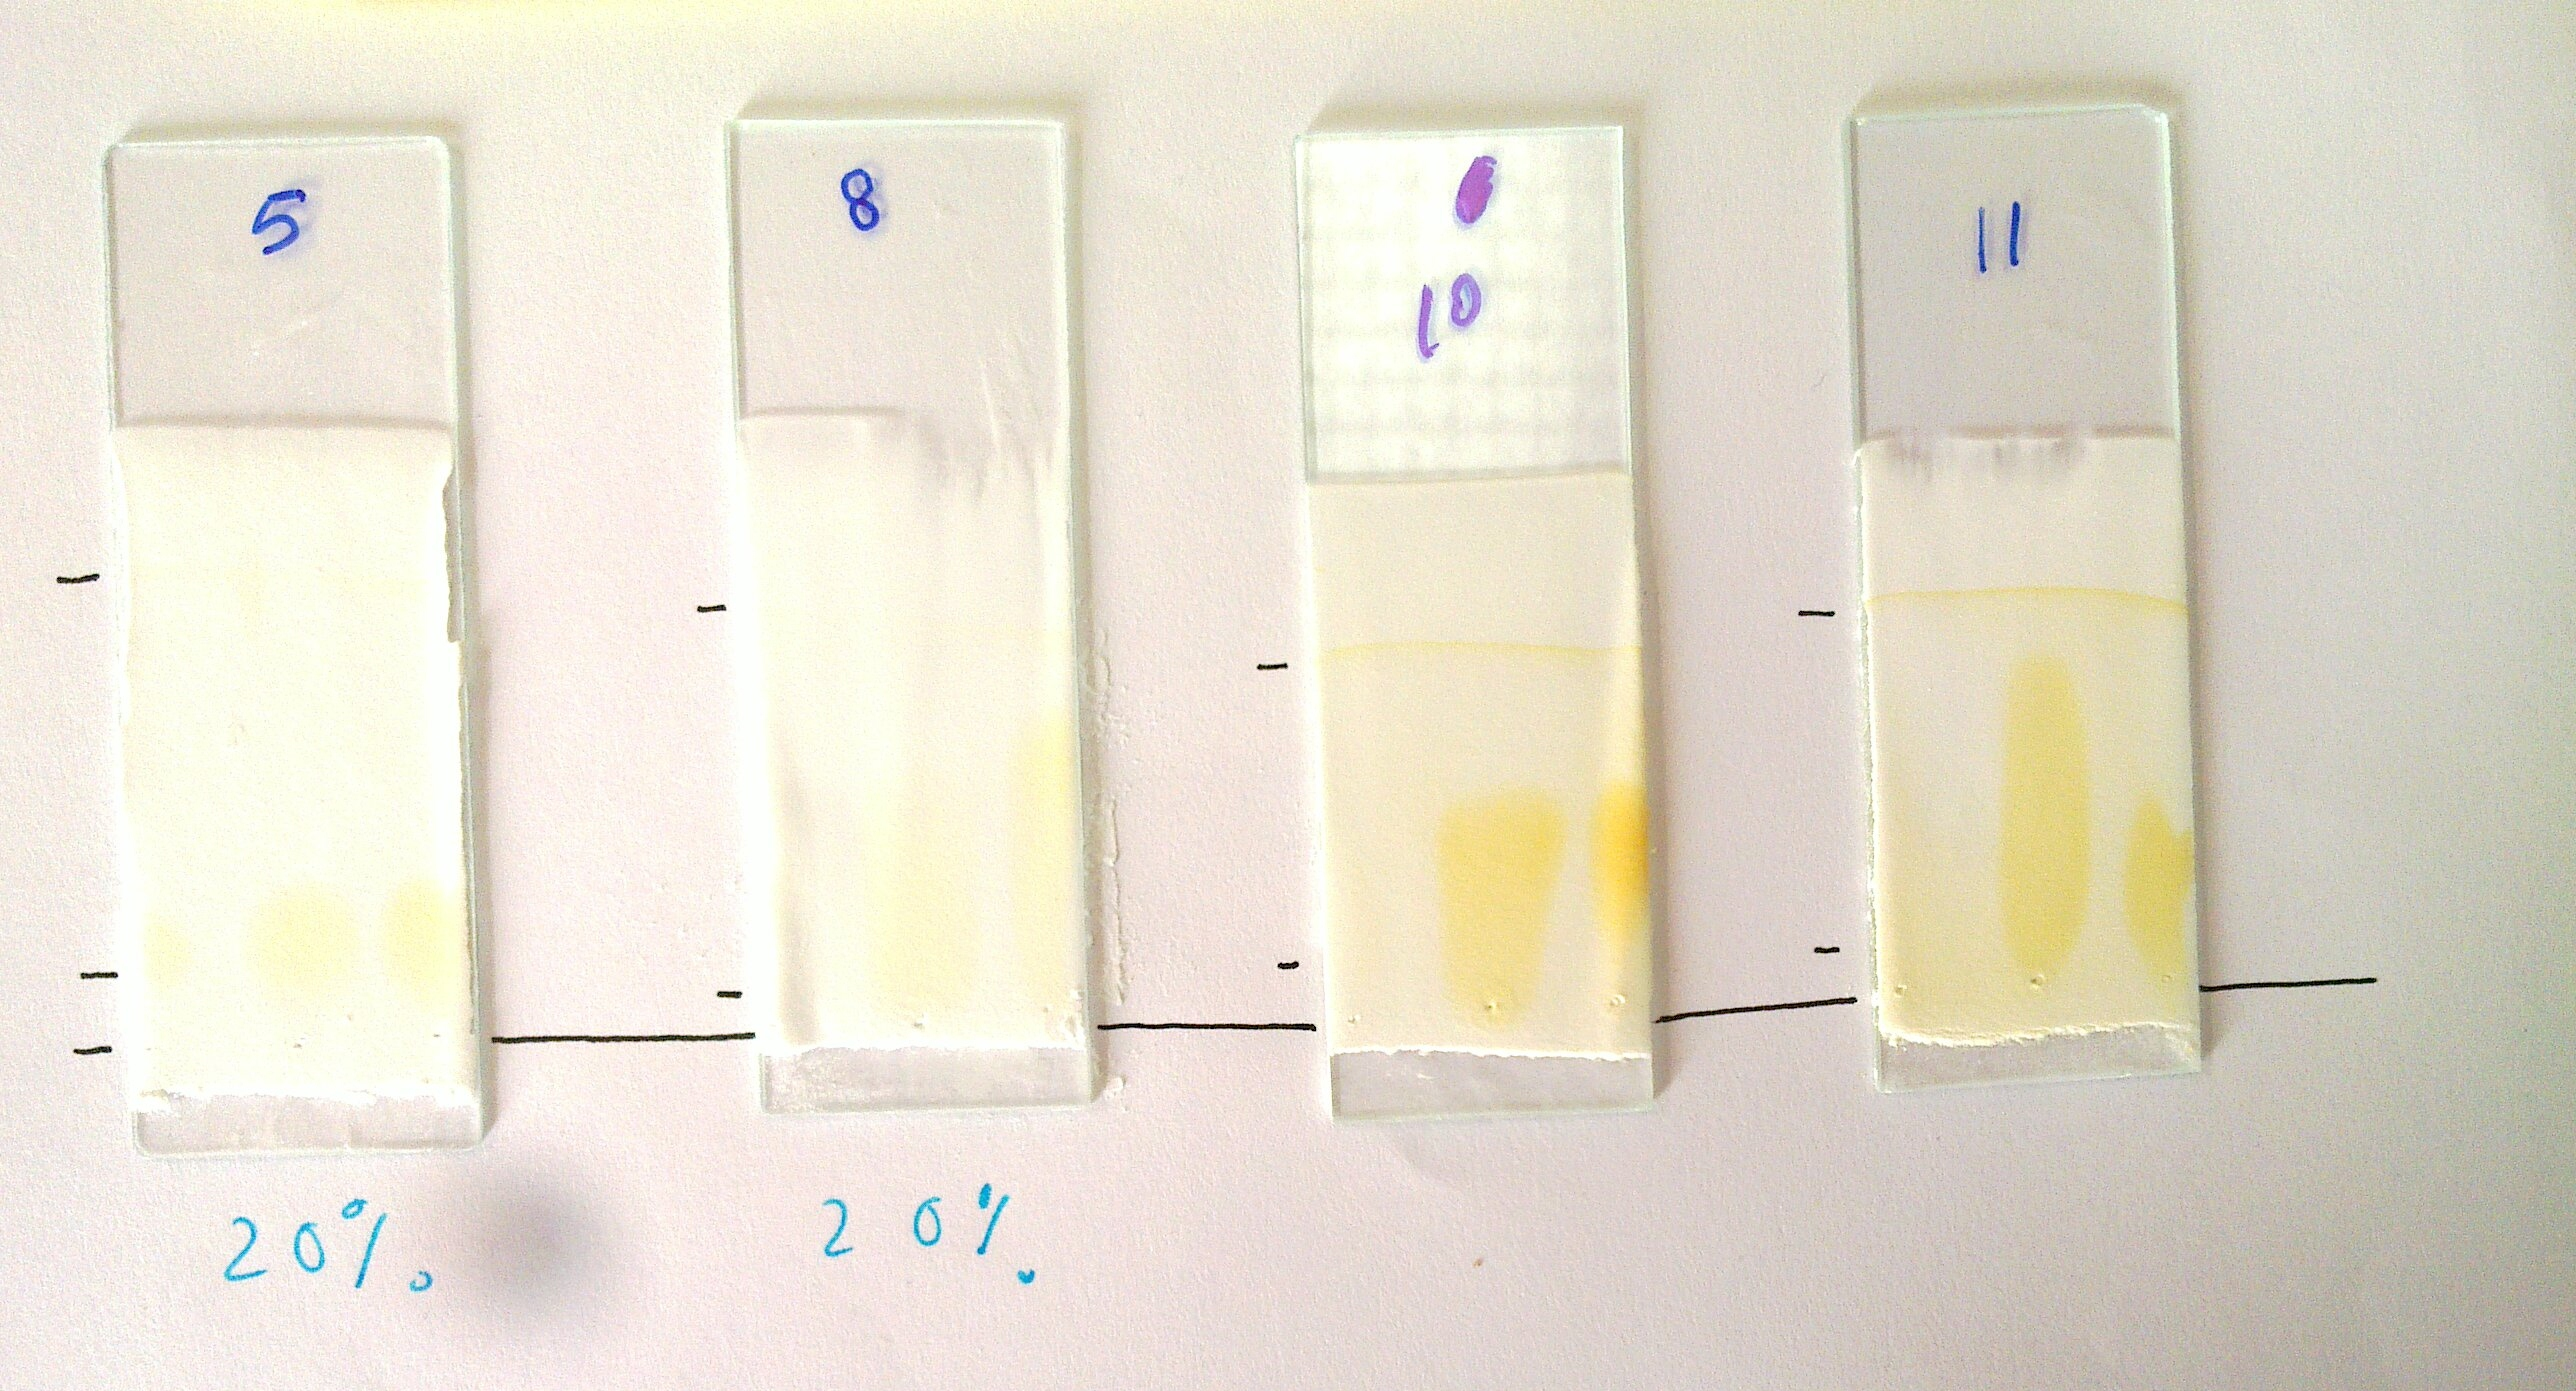
\includegraphics[width=1.2\linewidth]{gfx/e3_second}
		\end{center}
	\caption[TLC plates for the rest of the test tubes]{\label{e3_second}}
	\end{figure}


\section{Precaution}
	Precautions are same as those in the previous experiment, viz.
	\begin{enumerate}
		\item The slurry shouldn't be very thick
		\item Cover the beakers with a watch glass to ensure there's no loss of volatile substances (minimal that is)
		\item The coating is very fragile, thus the TLC plates must be handled with caution
	\end{enumerate}	
	Further,
	\begin{enumerate}
		\item We've to ensure there aren't any air bubbles in the column created, by tapping it enough.
		\item The hexane level shouldn't drop below the silica column's top, else cracks would begin to appear.
		\item Ensure the test tubes aren't cracked. \marginpar {\Bart One of our test tubes was infact cracked from the bottom and we lost that volume of the recovered compound.}
	\end{enumerate}
\section{Acknowledgements}
I thank Dr. R Vijaya Anand for his guidance during the experiment. I also acknowledge the contribution of my lab partners, Saumya, Vivek, Prashansa and Srijit for performance of the same, especially for being able to work in harmony, despite being a large group of five. I also thank our PhD guide for demonstrating the experiment and her assistance in general, with performance of the same.